\chapter{Background and Related Work} % (fold)
\label{cha:Related_Work}
\section{Twitter}
Twitter is a mircoblogging service. Now there are more than 140 million active users\footnote{https://blog.Twitter.com/2012/Twitter-turns-six}. User can publish short messages within 140 characters aka tweets.
\subsection{Retweet}
A retweet is re-posting of a tweet by other users. One way of retweet is using RT at the beginning of the tweet which is retweeted. The other way is using "retweet button" which is officially launched by Twitter after 2015. The difference between these two retweet is tweets are retweeted by "retweet button" can't be searched by Twitter's searching interface, but manually retweets with RT keyword can. So in our work retweet means the tweets are retweeted manually. The number of how many times of this tweet has been retweeted is showed behind it.

\subsection{Mentions}
Mentions are in form like "@username" which are added in the text of tweet. The users are mentioned will receive the notification of this tweet on their homepage.
\subsection{Hashtags}
Mentions are in form like "\#topic". It means this tweet belongs to some topics.

\subsection{Favorite}
Favorites means how many users like this tweet. It is showed on the interface of Twitter
\subsection{Verified User}
Verified User means this account of public interest is authentic by Twitter. It is showed by a blue icon behind the name of the poster.
\subsection{Followers}
The followers of a user are accounts who receive this user's posting. The total number of followers can been seen in the profile of poster.
\subsection{Following}
The following are other accounts who follow this user. The total number of following can been seen in the profile of poster.
\subsection{Twitter API}
Twitter API is provided by Twitter\footnote{https://dev.twitter.com/overview/api} for developer. But the search API only return a sampling of recent Tweets published in the past 7 days\footnote{https://dev.twitter.com/rest/public/search}. We need the full stories of the events, so we crawled the data directly from the searching interface\footnote{https://twitter.com/search-home}.
\section{Credibility of Tweets } % (fold)
Titter has been used for reporting breaking news when emergency events happen like disaster (wenxian). But the people are likely to trust the news which post on traditional news website more than the news with same headline but posted on twitter. And Thomson's work shows that different crowds of people trust tweets basing on different kinds of sources.\cite{thomson2012trusting}.

 \section{Definition of Rumor}
 The definition of rumor in our work is unverified information spreading on Twitter over time. It is a set of tweets including the the sources, spreaders, retweets, doubting  tweets and the denying tweet. 
 \subsection{Rumor Event}
 If a rumor didn't widely spread and it could be harmless. So we more focused on the rumors which are widely spread and contain one or more bursty pikes during propagation. We call it "rumor event".
\subsection{Time Period of an Event}
\label{sec:Time_Period_of_an_Event}

The beginning of a rumor event is hard to define. As far as I  know there is related work which give us a approach to define the beginning of one rumor event. One reason is a rumor may be created serval years ago and kept exiting in Twitter, but it didn't attract the people's attention. However it can be triggered by other events and suddenly quickly spread as a bursty event.

For example, a rumor\footnote{http://www.snopes.com/robert-byrd-kkk-photo/} claimed that Robert Byrd was member of KKK. This rumor has been circulating in Internet for a while, as shown in figure \ref{fig:KKK_full} that almost every day there are several tweets talking about this rumor. But this rumor was triggered by a picture about Robert Byrd kissing Hillary Clinton in 2016 and twitter users suddenly notice this rumor and this rumor was bursty spread. So what we are really interested in is the hours around the bursty pike.
 
\begin{figure}[!h]
\centering
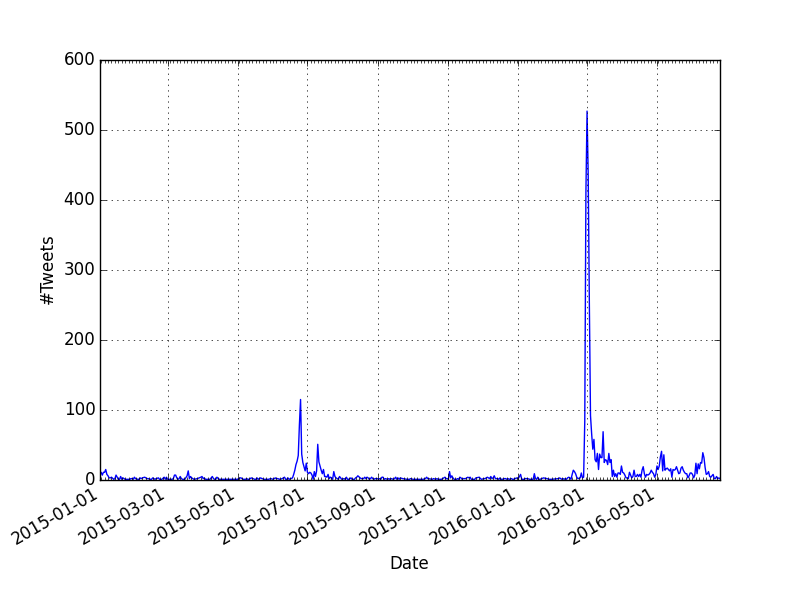
\includegraphics[width=0.7\columnwidth]{images/KKK_figure.png}
\caption{large scale tweet volume of event Robert Byrd}
\label{fig:KKK_full}
\end{figure}

 We defined the hour which has the most tweet's volume as $t_{max}$ and we want to detect the rumor event as soon as possible before its burst, so we define the time of the first tweet before $t_{max}$ within 48 hours as the beginning of this rumor event, marked as $t_{0}$. And the end time of events we defined as $t_{end}=t_0+48$. We show the tweet volume in figure \ref{fig:KKK_part} of the above rumor events after defined 48 hours time period.
  
\begin{figure}[!h]
\centering
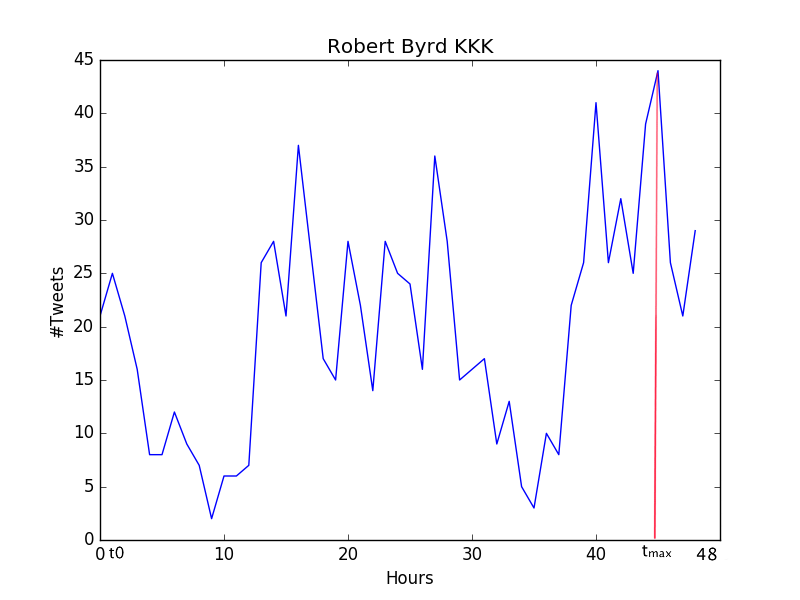
\includegraphics[width=0.7\columnwidth]{images/Robert_Byrd_KKK.png}
\caption{tweet volume of the rumor event of Robert Byrd after selected time period}
\label{fig:KKK_part}
\end{figure}



\section{Machine learning } % (fold)
\label{sec:Maschine_learning}
\subsection{Machine learning Overview} % (fold)

% Why are archives valuable
 Machine learning covers vast numbers of algorithms and has been successful applied in different field. The challenges of ML are finding the best model which is suitable for this task, fitting the parameters and selecting the features. 
 
Normally we split the ML methods into Supervised learning, Unsupervised learning and Reinforcement learning\cite{russell2003artificial}. 

The supervised learning is the most popular method of ML. It needs a set of inputs and a set of desired outputs. And the algorithm will learn to produce the correct output based on the new input. 

The unsupervised learning needs a set of inputs but no outputs. The algorithm will generate the outputs like clusters or patterns. The unsupervised learning task can be used for example when people can't label the outputs. 
\subsection{ Decision tree} % (fold)
\tikzset{
 sibling distance={6em},
  treenode/.style = {shape=rectangle, rounded corners,
                     draw, align=center,
                     top color=white, bottom color=blue!20},
  root/.style     = {treenode, font=\Large, bottom color=red!30},
  env/.style      = {treenode, font=\ttfamily\normalsize},
  dummy/.style    = {circle,draw},
      level distance          = 10em,
   edge from parent/.style = {draw, -latex}
}
\begin{figure}[!h]
\center
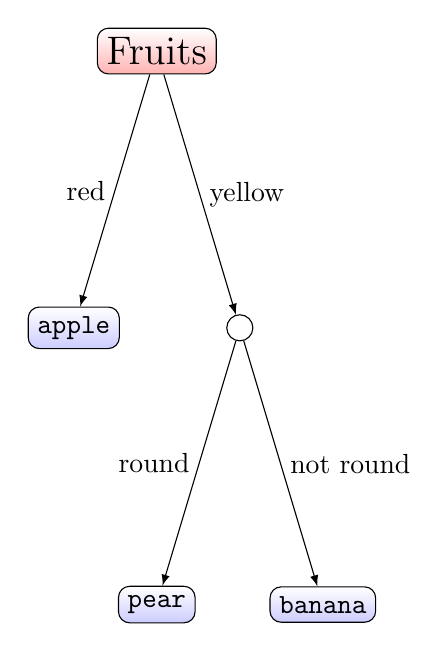
\begin{tikzpicture}
  
\node [root] {Fruits}
    child { node [env]{apple} edge from parent node [left] {red}}
    child { node [dummy] {}
      child { node [env] {pear} edge from parent node [left] {round}
      }
      child { node [env] {banana} edge from parent node [right] {not round}
      } edge from parent node [right] {yellow}
       };
\end{tikzpicture}
\label{fig:DeTree}
\end{figure}

\subsection{Random Forest (RF)} % (fold)
\label{random_forest}
Classification is a supervised data mining technique. Our work can be considered as a classification task. And the classification model is random forest.

RF is an algorithm of supervised learning which developed by Leo Breiman \cite{breiman2001random}. It's built by a set of classification trees \cite{breiman1984classification}. Each tree is trained by a small bootstrap sample of training set and while prediction each tree votes one single candidate. RF generates the result of prediction By taking the majority vote. 

For example we got task to classify pears and apples. We have the features are whether the fruit round, whether the fruit has seeds, whether the fruit red and whether the fruit is juicy. We build up a 3 trees random forest as the graph \ref{fig:randomforest}. Tree 1 randomly takes the subset of the features red and seeds and votes to apple. Tree 2 randomly takes the subset of the features red and seeds and votes to pear. Tree 3 randomly takes the subset of the features round and red and votes to apple. The most vote is apple, so the output of RF is apple.

\begin{figure}[!h]
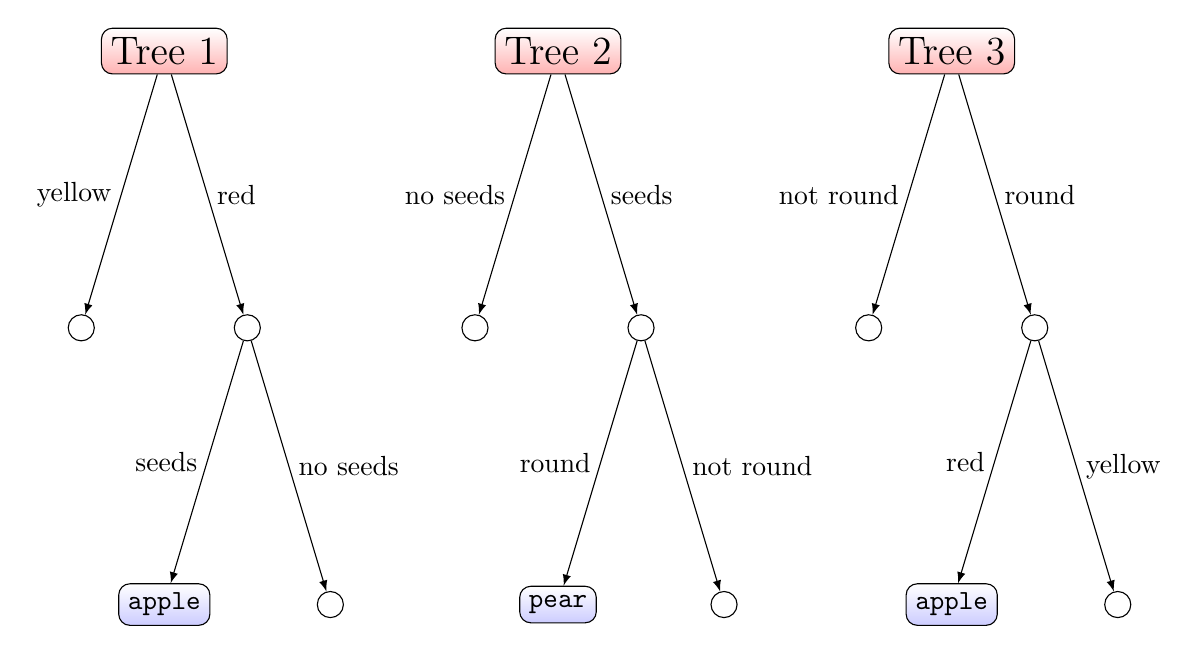
\begin{tikzpicture}
 \begin{scope} 
\node [root] {Tree 1}
      child { node [dummy] {} edge from parent node [left] {yellow}}
    child { node [dummy] {}
      child { node [env] {apple} edge from parent node [left] {seeds}
      }
      child { node [dummy] {} edge from parent node [right] {no  seeds}
      } edge from parent node [right] {red}
       };
       
       \end{scope}

  \begin{scope}[xshift=5cm]
\node [root] {Tree 2}
    child { node [dummy] {} edge from parent node [left] {no  seeds}}
    child { node [dummy] {}
      child { node [env] {pear} edge from parent node [left] {round}
      }
      child { node [dummy] {} edge from parent node [right] {not round}
      } edge from parent node [right] {seeds}
       };
  \end{scope}
  \begin{scope}[xshift=10cm]
\node [root] {Tree 3}
     child { node [dummy] {} edge from parent node [left] {not   round}}
    child { node [dummy] {}
      child { node [env] {apple} edge from parent node [left] {red}
      }
      child { node [dummy] {} edge from parent node [right] {yellow}
      } edge from parent node [right] {round}
       };
  \end{scope}
\end{tikzpicture}
  \caption{An example of random forest with 3 trees}
\label{fig:randomforest}
\end{figure}


Because RF uses a random subset of features instead of the best features in every node, so it can avoid the overfitting\cite{breiman2001random}. 

Another benefit of RF is that it can return the \textbf{features' importance}. RF is built up by a subset of training data. If there are N trees, RF will take N times bootstrap sampling. So some features we didn't select to use for training the model. The data we didn't selected we call it out-of-bag (OOB) data. In the above example the feature whether the fruit is juicy didn't join the construction the Trees, so it is a OOB data. These data can be use for validating the model and the output is OBB error $E_{oob}(G) = \frac {1}{N} \sum_{n=1}^{N}err(y_n,G_{n}^-(X_n))$ with $X_n$ are features only in OOB. At last we get the importance of feature by permuting one feature to random numbers. $importance(i)= E_{oob}(G)-E_{oob}^{p}(G)$ where $E_{oob}^{p}(G)$ is the OBB error after permuting a feature. The more performance drop down, that means the more important this feature is. We use this method to measure the performance of features and evolute the models later.
\subsection{Recurrent neural network} % (fold)
A Recurrent neural network (RNN) is one of of class of neural network \ref{fig:NN}. The different between RNN and other neural network is there are connections between the hidden layers \ref{fig:RNN}, that makes the sequence of the input can also influence the network. For example people understand the words in one sentence based on the previous words, the normal neural network will ignore the previous inputs.
 
\begin{figure}[!h]
\center
\def\layersep{2.5cm}

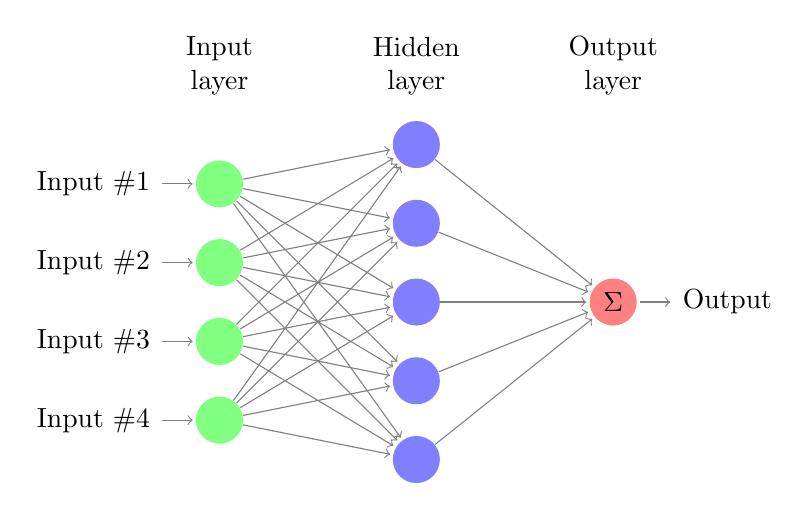
\begin{tikzpicture}[shorten >=1pt,->,draw=black!50, node distance=\layersep]
    \tikzstyle{every pin edge}=[<-,shorten <=1pt]
    \tikzstyle{neuron}=[circle,fill=black!25,minimum size=17pt,inner sep=0pt]
    \tikzstyle{input neuron}=[neuron, fill=green!50];
    \tikzstyle{output neuron}=[neuron, fill=red!50];
    \tikzstyle{hidden neuron}=[neuron, fill=blue!50];
    \tikzstyle{annot} = [text width=4em, text centered]

    % Draw the input layer nodes
    \foreach \name / \y in {1,...,4}
    % This is the same as writing \foreach \name / \y in {1/1,2/2,3/3,4/4}
        \node[input neuron, pin=left:Input \#\y] (I-\name) at (0,-\y) {};

    % Draw the hidden layer nodes
    \foreach \name / \y in {1,...,5}
        \path[yshift=0.5cm]
            node[hidden neuron] (H-\name) at (\layersep,-\y cm) {};

    % Draw the output layer node
    \node[output neuron,pin={[pin edge={->}]right:Output}, right of=H-3] (O)  {$\displaystyle\Sigma$};

    % Connect every node in the input layer with every node in the
    % hidden layer.
 
    \foreach \source in {1,...,4}
        \foreach \dest in {1,...,5}
            \path (I-\source) edge (H-\dest);

    % Connect every node in the hidden layer with the output layer
    \foreach \source in {1,...,5}
        \path (H-\source) edge (O);

    % Annotate the layers
    \node[annot,above of=H-1, node distance=1cm] (hl) {Hidden layer};
    \node[annot,left of=hl] {Input layer};
    \node[annot,right of=hl] {Output layer};
\end{tikzpicture}

   \caption{An example of 1 layer neural network}
\label{fig:NN}
\end{figure}



\begin{figure}[!h]
\center
\def\layersep{2.5cm}

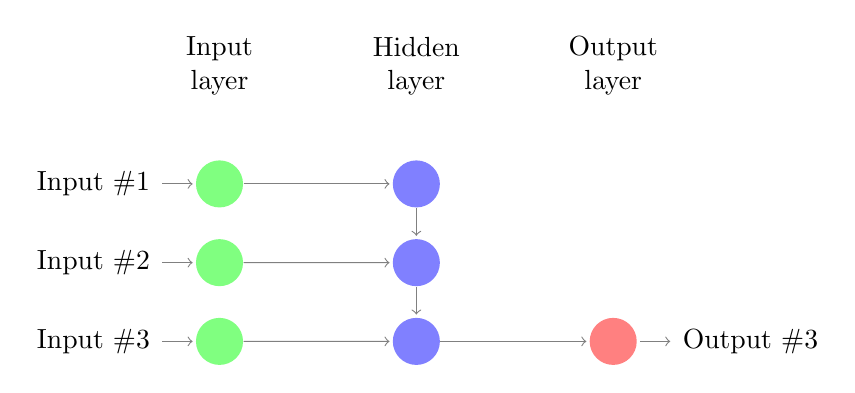
\begin{tikzpicture}[shorten >=1pt,->,draw=black!50, node distance=\layersep]
    \tikzstyle{every pin edge}=[<-,shorten <=1pt]
    \tikzstyle{neuron}=[circle,fill=black!25,minimum size=17pt,inner sep=0pt]
    \tikzstyle{input neuron}=[neuron, fill=green!50];
    \tikzstyle{output neuron}=[neuron, fill=red!50];
    \tikzstyle{hidden neuron}=[neuron, fill=blue!50];
    \tikzstyle{annot} = [text width=4em, text centered]

    % Draw the input layer nodes
    \foreach \name / \y in {1,...,3}
    % This is the same as writing \foreach \name / \y in {1/1,2/2,3/3,4/4}
        \node[input neuron, pin=left:Input \#\y] (I-\name) at (0,-\y) {};

    % Draw the hidden layer nodes
    \foreach \name / \y in {1,...,3}
        \path[yshift=0cm]
            node[hidden neuron] (H-\name) at (\layersep,-\y cm) {};

    \foreach \name / \y in {3,...,3}
    % This is the same as writing \foreach \name / \y in {1/1,2/2,3/3,4/4}
        \node[output neuron,pin={[pin edge={->}]right:Output  \#\y}, right of=H-\y] (O-\y) {};

     % Connect every node in the input layer with every node in the
    % hidden layer.
 
    \foreach \source in {1,...,3}
             \path (I-\source) edge (H-\source);
     \path (H-3) edge (O-3);

     % Connect every node in the hidden layer with the output layer
        
     \path  (H-1) edge    (H-2);
     \path  (H-2) edge    (H-3);

     % Annotate the layers
    \node[annot,above of=H-1, node distance=1.5cm] (hl) {Hidden layer};
    \node[annot,left of=hl] {Input layer};
    \node[annot,right of=hl] {Output layer};
\end{tikzpicture}

   \caption{multi-input single-output Recurrent neural network}
\label{fig:RNNMS}
\end{figure}



\begin{figure}[!h]
\center
\def\layersep{2.5cm}

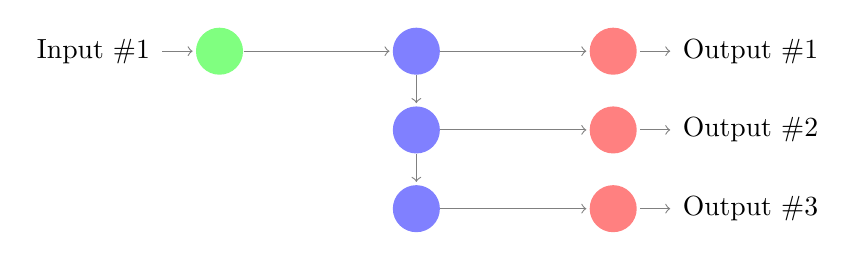
\begin{tikzpicture}[shorten >=1pt,->,draw=black!50, node distance=\layersep]
    \tikzstyle{every pin edge}=[<-,shorten <=1pt]
    \tikzstyle{neuron}=[circle,fill=black!25,minimum size=17pt,inner sep=0pt]
    \tikzstyle{input neuron}=[neuron, fill=green!50];
    \tikzstyle{output neuron}=[neuron, fill=red!50];
    \tikzstyle{hidden neuron}=[neuron, fill=blue!50];
    \tikzstyle{annot} = [text width=4em, text centered]

    % Draw the input layer nodes
    \foreach \name / \y in {1,...,1}
    % This is the same as writing \foreach \name / \y in {1/1,2/2,3/3,4/4}
        \node[input neuron, pin=left:Input \#\y] (I-\name) at (0,-\y) {};

    % Draw the hidden layer nodes
    \foreach \name / \y in {1,...,3}
        \path[yshift=0cm]
            node[hidden neuron] (H-\name) at (\layersep,-\y cm) {};

    \foreach \name / \y in {1,...,3}
    % This is the same as writing \foreach \name / \y in {1/1,2/2,3/3,4/4}
        \node[output neuron,pin={[pin edge={->}]right:Output  \#\y}, right of=H-\y] (O-\y) {};

     % Connect every node in the input layer with every node in the
    % hidden layer.
 
    \foreach \source in {1,...,1}
             \path (I-\source) edge (H-\source);
    \foreach \source in {1,...,3}
             \path (H-\source) edge (O-\source);

     % Connect every node in the hidden layer with the output layer
        
     \path  (H-1) edge    (H-2);
     \path  (H-2) edge    (H-3);

     % Annotate the layers
   % \node[annot,above of=H-1, node distance=1.5cm] (hl) {Hidden layer};
  %  \node[annot,left of=hl] {Input layer};
  %  \node[annot,right of=hl] {Output layer};
\end{tikzpicture}

   \caption{single-input multi-output Recurrent neural network}
\label{fig:RNNSM}
\end{figure}

\begin{figure}[!h]
\center
\def\layersep{2.5cm}

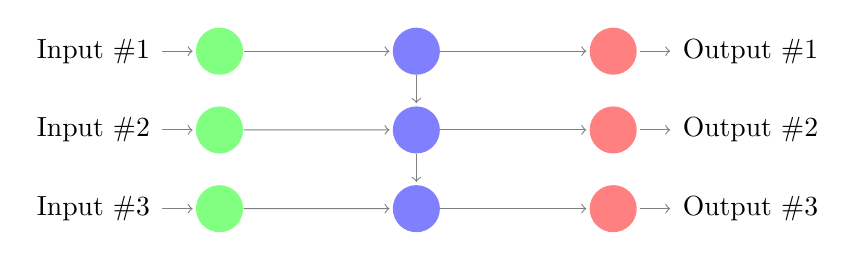
\begin{tikzpicture}[shorten >=1pt,->,draw=black!50, node distance=\layersep]
    \tikzstyle{every pin edge}=[<-,shorten <=1pt]
    \tikzstyle{neuron}=[circle,fill=black!25,minimum size=17pt,inner sep=0pt]
    \tikzstyle{input neuron}=[neuron, fill=green!50];
    \tikzstyle{output neuron}=[neuron, fill=red!50];
    \tikzstyle{hidden neuron}=[neuron, fill=blue!50];
    \tikzstyle{annot} = [text width=4em, text centered]

    % Draw the input layer nodes
    \foreach \name / \y in {1,...,3}
    % This is the same as writing \foreach \name / \y in {1/1,2/2,3/3,4/4}
        \node[input neuron, pin=left:Input \#\y] (I-\name) at (0,-\y) {};

    % Draw the hidden layer nodes
    \foreach \name / \y in {1,...,3}
        \path[yshift=0cm]
            node[hidden neuron] (H-\name) at (\layersep,-\y cm) {};

    \foreach \name / \y in {1,...,3}
    % This is the same as writing \foreach \name / \y in {1/1,2/2,3/3,4/4}
        \node[output neuron,pin={[pin edge={->}]right:Output  \#\y}, right of=H-\y] (O-\y) {};

     % Connect every node in the input layer with every node in the
    % hidden layer.
 
    \foreach \source in {1,...,3}
             \path (I-\source) edge (H-\source);
    \foreach \source in {1,...,3}
             \path (H-\source) edge (O-\source);

     % Connect every node in the hidden layer with the output layer
        
     \path  (H-1) edge    (H-2);
     \path  (H-2) edge    (H-3);

     % Annotate the layers
  %  \node[annot,above of=H-1, node distance=1.5cm] (hl) {Hidden layer};
  %  \node[annot,left of=hl] {Input layer};
   % \node[annot,right of=hl] {Output layer};
\end{tikzpicture}

   \caption{multi-input multi-output Recurrent neural network}
\label{fig:RNNMM}
\end{figure}

\section{Spark } % (fold)
\section{tensorflow } % (fold)
\section{LM fitting} % (fold)


\section{Related Work } % (fold)
People research on Twitter for a long time and there are a lots directions  to study this complex social network like event detection\cite{kimmey2015twitter}, spam detection \cite{ahmed2012mcl} \cite{wang2010don} or sentiment detection\cite{barbosa2010robust}. These work are similar with our task rumor detection but still contain many differences.

People first studied on rumors in psychology area for years \cite{allport1947psychology} \cite{sunstein2014rumors}.
But Twitter becomes an important platform for people sharing and exchanging information including rumors, the detection of misinformation on twitter turns to be a trending researching topic. 

Researcher first began from studying rumor spreading during several special events like natural disasters\cite{oh2010exploration} \cite{tanaka2012transmission} or terrorist attacks \cite{starbird2014rumors}. But these results are not general enough to other types of rumors. Our data includes sports, politic, entertainment, also natural disasters and other kinds of rumors. 

Carlos Castillo researched the information credibility on Twitter\cite{mendoza2010twitter} \cite{castillo2011information}\cite{gupta2014tweetcred}. But his work is more about people opinion (trustful or not) to a tweet not the credibility of tweet itself. But it still a good start of resolving problem. Lots of other works are based on Castillo's work \cite{yang2012automatic} \cite{liu2015real} and used different set of features. 

There are rencent researches based on the propagation of rumor on Sina Weibo\cite{yang2012automatic} \cite{wu2015false}, but twitter doesn't contain such detail of propagation like Weibo, so these work are useless for us. 

Liu's work \cite{wu2015false} focused on one type of rumor "the false photos" on social network not the general type of rumors.  

Xiaomo claimed their system is the first real time rumor debunking system on Twitter \cite{liu2015real}. But their work are similar with above other previous works, they use the static features of rumors and ignored the feature's changing over time during the event spreading on the social network which can be seen in figure \ref{fig:Url5000} and \ref{fig:largecity}. The fraction of tweets containing url with top 5000 domain and the fraction of poster living in large city which are both constantly changing. But one feature called "crowd wisdom" is an new idea and we use it in our work.

\begin{figure}[!h]
\centering
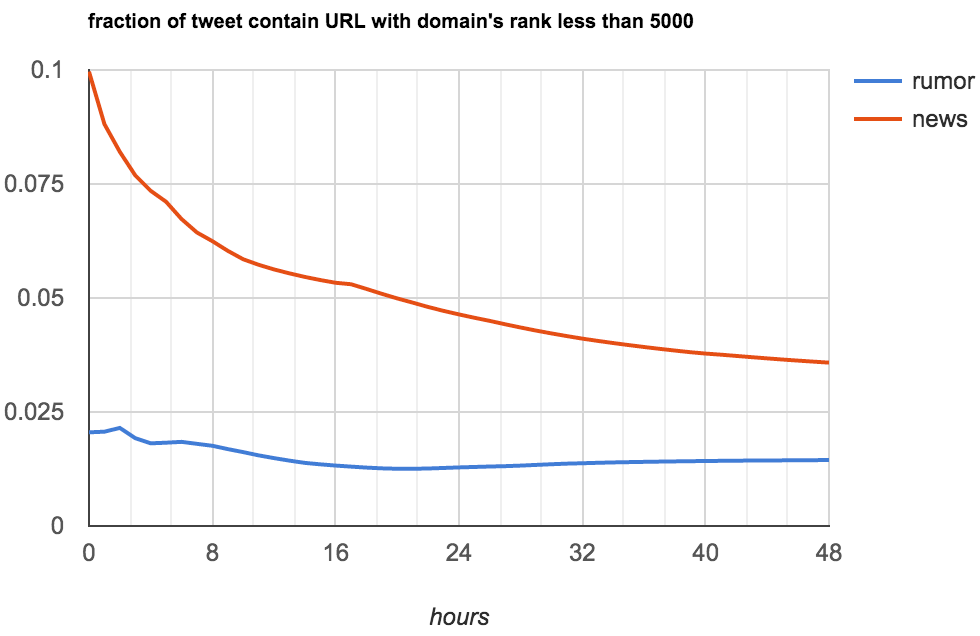
\includegraphics[width=0.52\columnwidth]{images/url5000.png}
\caption{The fraction of tweets containing url with top 5000 domain}
\label{fig:Url5000}
\end{figure}
\begin{figure}[!h]
\centering
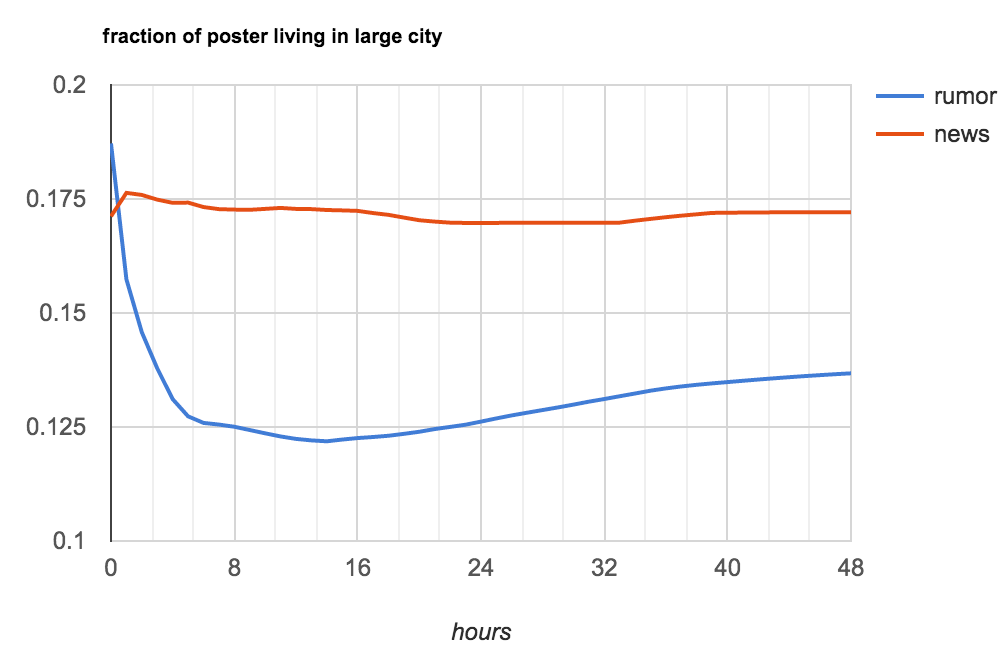
\includegraphics[width=0.52\columnwidth]{images/largecity.png}
\caption{The fraction of poster living in large city}
\label{fig:largecity}
\end{figure}

\newpage
Other researchers used propagation models like SpikeM \cite{kwon2013prominent} and SEIZ models \cite{jin2013epidemiological} to capture the tweet's volume changing over time, but they didn't use other features into time series model. And these features can't show the effect in the early stage of rumor spreading. We can provide it in the last section(wenxian).

J Ma used Recurrent Neural Networks for rumor detection \cite{madetecting}, as the same disadvantage of the other Neural Networks models, the process of model's training is black box to us, so we can't know way we got this result. In our case we can't get the evidences to convince people why the detected event is more likely to be a rumor or rather than a breaking news. 

Another work from J Ma used a time series model called Dynamic Series-Time Structure \cite{ma2015detect} to capture the variation of features. But they only used the features of social content and they didn't further explain how the performances of features change over time or how do they improve the performance of the model in first few hours after the events beginning.  We use their Series-Time Structure with our extended data and we will show how do these features change during time.

\chapter{Data Collection} % (fold)
\label{cha:Data_Collection}
We collected rumor stories from a rumor tracking website \textbf{snopes.com}. We crawled 4300 stories from the website and we manually constructed 130 queries. The approach of constructing queries is mainly following the work(wenxian). The regular expression of a query is $(Object \& Subject \& Description(Description1||Description2||...))$
for example a story is about Obama removing a flag in pearl harbor. Object is Obama, subject is flag and its synonym like flags, flagpole. Description is remove and its synonym removes, removed, removal, removing, "token down" or a url about this rumor "Departed.co". In this case there is a proper noun "pearl harbor" is also useful. Finally we transfer the regex to Twitter's query: obama (flag OR flags OR flagpole) (remove OR removes OR removed OR removal OR removing OR "token down" OR "Departed.co") pearl harbor.



We collect news stories for the data of (wenxian). We crawled average 50\% of them and we selected events with the most coverage and minimal 100 tweets. 

After we crawled and parsed the whole timeline of an events. We detect the 48 hours time period of the burst in the way we mentioned in section \ref{sec:Time_Period_of_an_Event}. We crawled the homepage of poster of the tweets in the event time period total 133,396 users. We also extracted 11,038 domains which are contained in the tweets in the 48 hours time period and we crawled these domains' catalogs in bluecoat.com \footnote{http://sitereview.bluecoat.com/sitereview.jsp\#/?search=bbc.com}, ranks in alexa.com\footnote{http://www.alexa.com/siteinfo/bbc.com} and WOT score in \footnote{https://www.mywot.com/en/api}. 

We use Beautiful Soup as the html parsing library to parse the Twitter timeline pages and the users' homepage \footnote{https://www.crummy.com/software/BeautifulSoup/bs4/doc/}. Beautiful Soup is a Python library for pulling data out of HTML and XML files. For increasing the speed of parsing html and extracting features from raw data, we use Spark\footnote{http://spark.apache.org/} technology, because it can simply manage multithread and its MapReduce in memory technology makes the calculation much quicker.  

\chapter{Single Tweet's Creditability Scoring Model} % (fold)
\label{cha:single_tweet_creditbility_scoring_model}
Most of the pervious researches are focusing on event level rumors and claims taht the task of classification for individual tweet is not reliable \cite{liu2015real} \cite{ma2015detect} \cite{zhao2015enquiring}, because a single tweet is to short to contains engough features. But Carlos Castillo designed a single tweet's creditability rank system Tweetcred \cite{gupta2014tweetcred}. So we think it is still enable to build up a single tweet creditability model. And we were inspired by the (wenxian) work that we may use nn() without handcrafted features to build up the single tweet's creditability model which in later experiments outputs a better performance.   
\section{Single Tweet's Creditability Model with handcrafted features} % (fold)
First we follow Castillo's \cite{gupta2014tweetcred} idea to implement a single tweet's creditability model with handcrafted features and we test it with decision trees, decision forest and SVM. But the performance of each model are not good enough. 

\subsection{Features}
We use a collection of features major from  Castillo's Tweetcred system\cite{gupta2014tweetcred} totally 27 features in table \ref{tab:single_features}. These features can be extracted directly from Twitter interface without third part website. 
\subsubsection{Text Features}
The Text features capture the content of the text of the tweets. There are 16 Text features. 
\textbf{Sentiment Features} are included in text features.
We used the python natural language Toolkit (nlTK) \footnote{http://www.nltk.org/} to analyze the tweets' sentiment and extract the features: the NumPositiveWords, NumNegativeWords and Polarityscores. Polarity scores is a float for sentiment strength of one tweet\footnote{http://www.nltk.org/api/nltk.sentiment.html} $Polarity\_scores = \frac {1}{N}    \sum_{0}^{n} {Polarity(token_n)}$.

\subsubsection{User Features} We selected total 5 features of the poster. These features are extracted directly from the twitter interface as in figure \ref{fig:UserSample}. ReputationScore is defined as the ratio between \#Friends over \# Followers. $ReputationScore = \frac {\#Friends }{\#Friends +\#Followers}$.
\begin{figure}[!h]
\centering
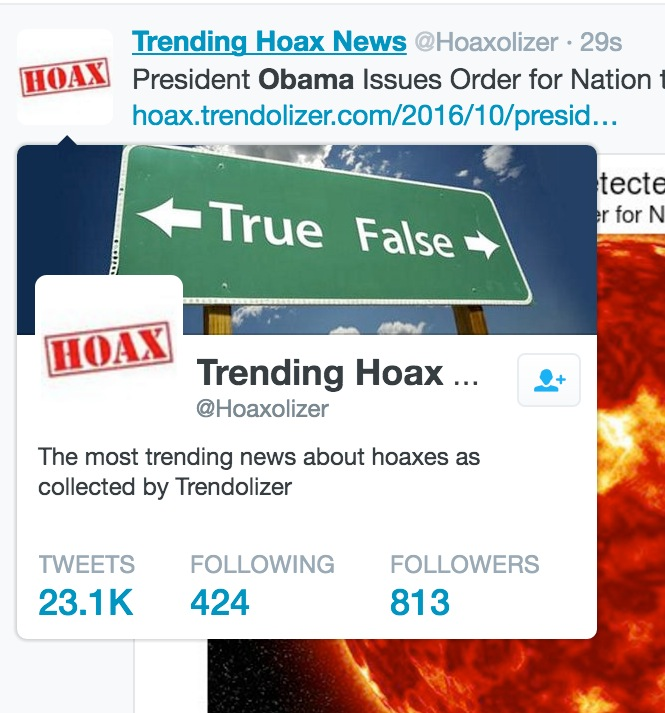
\includegraphics[width=0.55\columnwidth]{images/UserSample.png}
\caption{Sample of Users' Information on Twitter Interface}
\label{fig:UserSample}
\end{figure}

\subsubsection{Twitter Features} Twitter Features are the features of twitter's special functions. It includes Hashtag, Mention, Number of URLs, Number of retweeted and whether this tweet is retweet (contains RT as keywords or \emph{"QuoteTweet-innerContainer u-cf js-permalink js-media-container"} as the CSS class of the tweet in html).


\begin{table*}[!h]
\small
\centering
\scalebox{0.8}{
 \begin{tabular}{@{}lllllll@{}}
 \toprule
 \textbf{Category} & \textbf{Feature} & \textbf{Description}\\ \midrule
 Twitter Features& Hashtag & Whether the tweet contains \#hashtag\\
 		& Mention & Whether the tweet mentions others @user\\
 		& NumUrls & \# url in the tweet \\
 		& Retweets & How many times this tweet has been retweeted \\ 
 		& Isretweet & Whether this tweet is retweeted from others\\
\midrule
 Text Features & LengthofTweet & The length of tweet\\
    & NumofChar & \# of individual characters \\
   & Capital &  Fraction of characters in Uppercase \\
   & Smile & Whether this tweet contains :->, :-), ;->, ;-)\\
   & Sad & Whether this tweet contains :-<, :-(, ;->, ;-(\\
   & NumPositiveWords & \# of positive words\\
   & NumNegativeWords & \# of negative words\\
   & Polarityscores & polarity scores of the Tweet\\
   & Via & Whether this tweet contains via\\
   & Stock & Whether this tweet contains \$ \\
   & Question & Whether this tweet contains ? \\
   & Exclamation & Whether this tweet contains ! \\
   & QuestionExclamation & Whether this tweet contains multi Question or Exclamation mark \\ 
   & I & Whether this tweet contains  first pronoun like I, my, mine, we, our   \\
   & You & Whether this tweet contains second pronoun like U, you, your, yours \\ 
   & HeShe & Whether this tweet contains third pronoun like he, she, they, his, etc. \\\midrule
   User Features & Followers  & \# of followers\\
 	& Friends  & \# of friends\\
 	& Tweets  & \# of tweets which are posted by this user\\
 	& Description  & Whether this user has description\\
 	& Verified  & Whether this user is a verified user\\
 	& ReputationScore & Ratio between \#Friends over (\# Followers + \#Friends)\\
 \bottomrule
 \end{tabular}}
 \caption{Features for Single Tweet's Creditability Scoring Model}
 \label{tab:single_features}
\end{table*}
 \newpage

\subsection{Classification Methods}
Most of existing researches use SVM, Random Forest and DT. We test our data also with these 3 models.  We implement these 3 model with scikit-learn library\footnote{scikit-learn.org/}. We shuffled the 260 events and split them into 10 subset, we uses them for 10 times cross-validation. We show the parameters after optimization for each model them in table \ref{tab:single_model_para}.

\begin{table*}[!h]
 \centering
\scalebox{0.8}{
 \begin{tabular}{@{}lllllll@{}}
 \toprule
 \textbf{Model} & \textbf{Parameters} & \textbf{Value} \\ \midrule
 Random Forest & Number of Trees & 200\\ \midrule
 SVM & kernel  & radial basis function\\
 	& penalty parameter of the error term  & 2.0\\
 	& gamma  & $\frac{1}{27}$\\ \midrule
 Decision Trees & criterion & gini \\ \bottomrule
 \end{tabular}}
 \caption{Parameters of Classification models}
 \label{tab:single_model_para}
\end{table*}

 We show the results in the table \ref{tab:single_result}. The  best model with the highest accuracy is RF, but it reaches only 64.87\% and the other two models are even worse, so it is clear to see with manually handcrafted features, one single tweet is difficulty to be classified.  
 \begin{table*}[!h]
 \centering
\scalebox{1.1}{
 \begin{tabular}{@{}lllllll@{}}
 \toprule
 \textbf{Model} & \textbf{Accuracy} \\ \midrule
 Random Forest & \textbf{0.6487 }\\
 SVM &  0.5802\\
 Decision Trees &  0.5774\\ \bottomrule
 \end{tabular}}
 \caption{Prediction Accuracy of Different Single Tweet's Creditability Scoring Models}
 \label{tab:single_result}
\end{table*}

 And we rank the features using the features importance which we mentioned in section \ref{random_forest}, showing in table \ref{tab:Features_Importance}. The best feature is polarity scores of sentiment. It means that there is a big bias between the rumors tweets and the tweets real events. It was mentioned by previous work \cite{allport1947psychology} where he gathered a large rumors collection during WW2 which are printed in the Boston Heralds Rumor Clinic. He summarized rumors as several types:  pipe-dream, fear and aggression. The most researches believe that rumors mostly contain negative sentiment and polarity \cite{sunstein2014rumors}\cite{kwon2013aspects}. In our study average polarity score of news event is -0.066 and average polarity score of rumors is -0.1393 ,it means that rumors contain more negative sentiment. 
 
 And we usually think the verified users may have less possibility to be involved in the rumors' spreading, but the result shows that the verified users may be not really trustful like we thought. And "Isreweet" feature is neither a good feature which means the possibility of people retweeting the rumors or true events are similar.
 
  
 

\begin{table*}[!h]
 \centering
\scalebox{1}{
\begin{tabular}{@{}lllllll@{}}
\toprule
\textbf{Feature} & \textbf{Feature Importance} \\ \midrule
PolarityScores	&	0.1460686474\\
Capital	&	0.09638447209\\
LengthofTweet  &	0.09283739724\\
Tweets  &	0.08750049577 \\
Friends  &	0.08065591431 \\
ReputationScore  &	0.08002109553 \\
Followers   &	0.07938657292 \\
NumOfChar	&	0.07659755102\\
Stock	&	0.04920394972\\
NumNegativeWords	&	0.03068379335\\
Exclamation	&	0.02304551015\\
numUrls	&	0.02124370609\\
NumPositiveWords	&	0.01976939973\\
Hashtag	&	0.01851408745\\
Mention	&	0.01596532677\\
Question	&	0.01486070376\\
Retweets	&	0.01349486577\\
I	&	0.0109471116\\
You	&	0.00998103276\\
HeShe	&	0.00774915859\\
UserDescription	&	0.007402174886\\
Via	&	0.005545157727\\
QuestionExclamation	&	0.005422123705\\
Isretweet	&	0.003240079497\\
Verified	&	0.003081752983\\
Smile	&	0.0003979192278\\
Sad	&	0\\ \bottomrule

\end{tabular}}
\caption{Features Importance}
\label{tab:Features_Importance}
\end{table*}

 \newpage
 \section{Single Tweet's Creditability Model without handcrafted features} 

As we showed in last section. The result of Single Tweet's Creditability Model with handcrafted features no matter with SVM, DT or RF is not so convincible. We may miss some important features we didn't mine out of the tweet. Inspired by the Lai and J Ma's works \cite{lai2015recurrent} \cite{madetecting} we test neural networks as the classifier to build up this system. It doesn't need to extract features from the raw data. So now we can think this task as a normal text classification task.
Based on the previous work we tested it with (wenxian) models: Basic tanh-RNN, 1-layer GRU-RNN as figure \ref{fig:1GRU} and 2-layer GRU-RNN as figure\ref{fig:2GRU} model.
\begin{figure}[!h]
\center
\def\layersep{2.5cm}

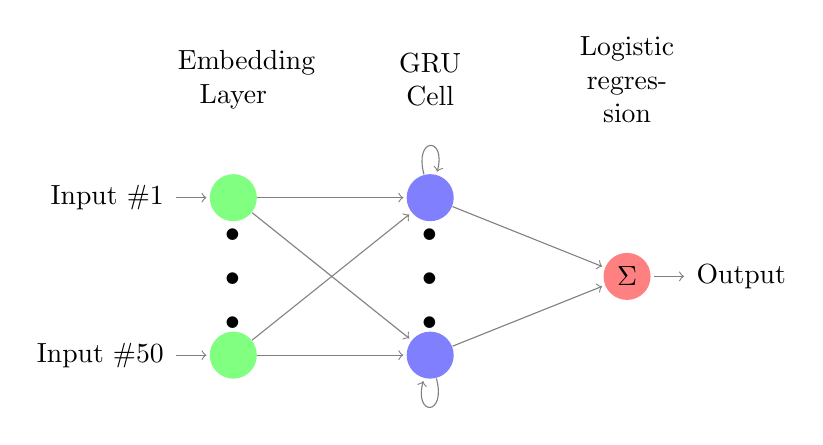
\begin{tikzpicture}[shorten >=1pt,->,draw=black!50, node distance=\layersep]
    \tikzstyle{every pin edge}=[<-,shorten <=1pt]
    \tikzstyle{neuron}=[circle,fill=black!25,minimum size=17pt,inner sep=0pt]
    \tikzstyle{input neuron}=[neuron, fill=green!50];
    \tikzstyle{output neuron}=[neuron, fill=red!50];
    \tikzstyle{hidden neuron}=[neuron, fill=blue!50];
    \tikzstyle{annot} = [text width=4em, text centered]
    \tikzstyle{neuron missing} = [draw=none,scale=4,text height=0.333cm , execute at begin node=\color{black}$\vdots$]
    % Draw the input layer nodes
     % This is the same as writing \foreach \name / \y in {1/1,2/2,3/3,4/4}
        \node[input neuron, pin=left:Input \#1] (I-1) at (0,-1) {};
        \node[input neuron, pin=left:Input \#50] (I-2) at (0,-3) {};
        \node[neuron missing,]  at (0,-2) {};

    % Draw the hidden layer nodes
         \node[hidden neuron] (H-2) at (\layersep,-3) {};
         \node[hidden neuron] (H-1) at (\layersep,-1) {};
        \node[neuron missing,]  at (\layersep,-2) {};

    % Draw the output layer node
    \node[ output neuron,pin={[pin edge={->}]right:Output},  xshift=5cm,yshift=-2cm] (O) {$\displaystyle\Sigma$};

    % Connect every node in the input layer with every node in the
    % hidden layer.
 
    \foreach \source in {1,...,2}
        \foreach \dest in {1,...,2}
            \path (I-\source) edge (H-\dest);

     % Connect every node in the hidden layer with the output layer
    \foreach \source in {1,...,2}
        \path (H-\source) edge (O);
       
     \path  (H-1) edge [loop above]  (H-1);
     \path  (H-2) edge [loop below]  (H-2);
    % Annotate the layers
    \node[annot,above of=H-1, node distance=1.5cm] (hl) {GRU Cell};
    \node[annot,left of=hl] {Embedding Layer};
    \node[annot,right of=hl] {Logistic regression};
\end{tikzpicture}
   \caption{1 layer GRU Recurrent neural network}
\label{fig:1GRU}
\end{figure}



\begin{figure}[!h]
\center
\def\layersep{1.8cm}

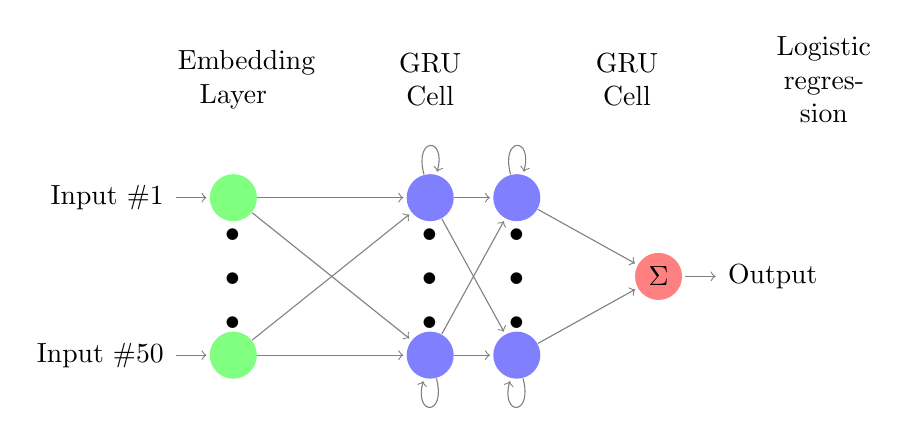
\begin{tikzpicture}[shorten >=1pt,->,draw=black!50, node distance=\layersep]
    \tikzstyle{every pin edge}=[<-,shorten <=1pt]
    \tikzstyle{neuron}=[circle,fill=black!25,minimum size=17pt,inner sep=0pt]
    \tikzstyle{input neuron}=[neuron, fill=green!50];
    \tikzstyle{output neuron}=[neuron, fill=red!50];
    \tikzstyle{hidden neuron}=[neuron, fill=blue!50];
    \tikzstyle{annot} = [text width=4em, text centered]
    \tikzstyle{neuron missing} = [draw=none,scale=4,text height=0.333cm , execute at begin node=\color{black}$\vdots$]
    % Draw the input layer nodes
     % This is the same as writing \foreach \name / \y in {1/1,2/2,3/3,4/4}
        \node[input neuron, pin=left:Input \#1] (I-1) at (0,-1) {};
        \node[input neuron, pin=left:Input \#50] (I-2) at (0,-3) {};
        \node[neuron missing,]  at (0,-2) {};

    % Draw the hidden layer nodes
         \node[hidden neuron] (H-2) at (\layersep,-3) {};
         \node[hidden neuron] (H-1) at (\layersep,-1) {};
        \node[neuron missing,]  at (\layersep,-2) {};
        
         \node[hidden neuron] (W-2) at (3.6,-3) {};
         \node[hidden neuron] (W-1) at (3.6,-1) {};
        \node[neuron missing,]  at (3.6,-2) {};

    % Draw the output layer node
    \node[ output neuron,pin={[pin edge={->}]right:Output},  xshift=5.4cm,yshift=-2cm] (O) {$\displaystyle\Sigma$};

    % Connect every node in the input layer with every node in the
    % hidden layer.
 
    \foreach \source in {1,...,2}
        \foreach \dest in {1,...,2}
            \path (I-\source) edge (H-\dest);
    \foreach \source in {1,...,2}
        \foreach \dest in {1,...,2}
            \path (H-\source) edge (W-\dest);
     \path  (W-1) edge [loop above]  (W-1);
     \path  (W-2) edge [loop below]  (W-2);


     % Connect every node in the hidden layer with the output layer
    \foreach \source in {1,...,2}
        \path (W-\source) edge (O);
       
     \path  (H-1) edge [loop above]  (H-1);
     \path  (H-2) edge [loop below]  (H-2);
    % Annotate the layers
    \node[annot,above of=H-1, node distance=1.5cm] (hl) {GRU Cell};
    \node[annot,left of=hl] {Embedding Layer};
    \node[annot,right of=hl] (h2) {GRU Cell};
    \node[annot,right of=h2]  {Logistic regression};

\end{tikzpicture}

   \caption{2 layer GRU Recurrent neural network}
\label{fig:2GRU}
\end{figure}


  \subsection{Data preparing} % (fold)
We use the same dataset as the above models and same shuffled sequence. The difference is the we feed only the text of each tweet to our neural network models. And we randomly take 10\% data from the training set to be the valid set for optimizing
 the parameters. 
 \subsection{First Layer: Embedding Layer}  
 The first layer is embedding layer which is same to both models. The size of embedding we set up as 50. The output of the layer will be a vector presenting the words. 
  \subsection{Hidden Layer: GRU and LSTM}  
  

\chapter{Time Seriers Rumor Detection Model} % (fold)
\label{cha:timr_seriers_rumor_model}
As we showed in figures \ref{fig:Url5000} and \ref{fig:largecity}, the features change during the the events' spreading over time. In order to capture these changes of the each features we use Dynamic Series-Time Structure (DSTS) which was presented in Ma's work \cite{ma2015detect}. In the an Event $E_{i}$ there is a set of tweets $tw_{ij}$ and we split them into different time intervals according to the creation time so that we can analyze the features in time series. We test the different classifiers with this model, we compare it with static features and in the end we rank all features and show their performance over time.
  \section{ Dynamic Series-Time Structure (DSTS)} 
   \subsection{Time Stamps Generation} 
   For an event $E_i$ we define $timeFirst_i$ as the start time of the event, $timeFirst_i$ as the time of last tweet of the event. We split the each tweet $tw_{ij}$ into N time intervals according to the creation time. The length of each time interval we define as follow: 
   
\begin{equation}
Interval(E_i)=\frac{\left \lceil { (timeLast_i-timeFirst_i) }\right \rceil}{N}
\end{equation}
And the index of time interval $TS(t_{ij})$ where a tweet $tw_{ij}$ which is created in time $t_{ij}$ should fall into, we define as follow :

\begin{equation}
TS(t_{ij})=\frac{\left \lfloor { (t_{ij}-timeFirst_i) }\right \rfloor}{Interval(E_i)}
\end{equation}

In our work $Interval(E_i)$ as we defined in section \ref{sec:Time_Period_of_an_Event} is one hour and N is constant 48 hours for each event.  
   
   \subsection{ Dynamic Series-Time Structure (DSTS)} 
Now we have all the time intervals of an event $E_i$ and we can generate a vector V($E_i$ ) of features in each time interval. And in order to capture the changes of feature over time we should no only model the features in individual time intervals but also we should model their difference between two time intervals. So the model of  DSTS is represented as:  

\begin{equation}
 V(E_i)=(\textbf{F}^D_{i,0}, \textbf{F}^D_{i,1},..., \textbf{F}^D_{i,N},\textbf{S}^D_{i,1},..., \textbf{S}^D_{i,N})
\end{equation}
where the $\textbf{F}^D_{i,t}$ is the feature vector in time interval t of event $E_i$.  $\textbf{S}^D_{i,t}$ is the difference between $\textbf{F}^D_{i,t}$ and $\textbf{F}^D_{i,t+1}$. V($E_i$ ) is the time series feature vector of the event $E_i$.
\begin{equation}
\textbf{F}^D_{i,t}=(\widetilde{ f}_{i,t,1},\widetilde{ f}_{i,t,2},...,\widetilde{ f}_{i,t,D})
\end{equation}

\begin{equation}
\textbf{S}^D_{i,t}=\frac{\textbf{F}^D_{i,t+1}-\textbf{F}^D_{i,t}}{Interval(E_i)}
\end{equation}
We use Z-score to normalize feature values which is implemented by sklearn.
\begin{equation}
\widetilde{f}_{i,t,k}=\frac{f_{i,t+1,k}-\overline{f}_{i,k}}{\sigma(f_{i,k})}
\end{equation}
where$f_{i,t,k}$ is the k-th feature in time interval t of the event $E_i$ in time interval t. $\overline{f}_{i,k}$ is the mean of the feature k of the event $E_i$ and $sigma(f_{i,k})$ is the standard deviation of the feature k over all time intervals. We skip this step when we use random forest because RF doesn't need feature normalization.

 \subsection{Features} 
 
 We use a collection of features based on previous works \cite{jin2013epidemiological}
\cite{mendoza2010twitter}\cite{castillo2011information}\cite{gupta2014tweetcred}\cite{yang2012automatic}\cite{liu2015real}\cite{madetecting}\cite{wu2015false}\cite{ma2015detect}. We extracted totally 49 features in table \ref{tab:full_features}. These features are not only extracted from Twitter interface but also other website like bluecoat.com we mentioned them in section \ref{cha:Data_Collection}. 
\subsubsection{Text Features}
\subsubsection{Twitter Features}
\subsubsection{User Features}
The list of large city \footnote{http://www.demographia.com/db-worldua.pdf}
\subsubsection{Epidemiological Modeling Features}
Jin's work is as far as we know the first people using epidemiological model to analyze rumors' prorogation on twitter \cite{jin2013epidemiological}. They fits the volume of the rumors and news events into two models SIS (Susceptible, Infected, Susceptible) and SEIZ (susceptible, exposed, infected, skeptic). 

\textbf{SIS} is one of the most popular epidemiological model. To adapt to the scenario of Twitter, we define a user who posts a tweet of relevant event as \textbf{I}nfected, a user who didn't we define as \textbf{S}usceptible. But unlikely as a normal epidemiological scenario infected nodes can be cured and return to be susceptible,  the user once posts a tweet of the certain events, he will be classified into the infected component forever. He can't be return susceptible class. At time t the total number of population is $\Delta N(t)= I(t) + S(t)$ where $I(t)$ is the size of infected population and  $S(t)$ is the size of susceptible population.  As shown in Figure \ref{fig:SIS}, SIS model works as follow:

\begin{figure}[!h]
\center
\def\layersep{2.5cm}
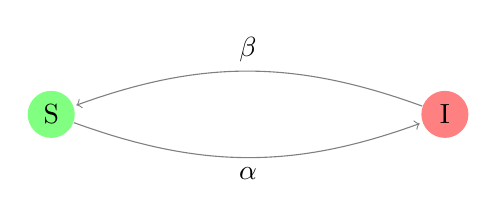
\begin{tikzpicture}[shorten >=1pt,->,draw=black!50, node distance=\layersep]
    \tikzstyle{every pin edge}=[<-,shorten <=1pt]
    \tikzstyle{neuron}=[circle,fill=black!25,minimum size=17pt,inner sep=0pt]
    \tikzstyle{input neuron}=[neuron, fill=green!50];
    \tikzstyle{output neuron}=[neuron, fill=red!50];
    % Draw the input layer nodes
     % This is the same as writing \foreach \name / \y in {1/1,2/2,3/3,4/4}
      \node[input neuron] (S) at (0,-1) {S};
     \node[ output neuron,  xshift=5cm,yshift=-1cm] (I) {I};
      \path  (I) edge [above, bend right=20]node [sloped,midway,above] {$\beta$} (S) ;
     \path  (S) edge [below, bend right=20] node [sloped,midway,below]{$\alpha $}(I) ;
    % Annotate the layers
 \end{tikzpicture}
   \caption{SIS Model}
\label{fig:SIS}
\end{figure}
	
\begin{itemize}
\item A user who posts tweets about the certain event is regarded as infected
\item A susceptible user has not tweeted about the certain event
\item A susceptible user may see the a tweet about the certain event from a infected users and he immediately retweets or posts a tweet about this events, and in that he turns himself to infected.
\item Susceptible user will remain susceptible until he contacts (via tweet) with infected person.
\end{itemize}
we show SIS model mathematical as follow:
\begin{equation}
\frac{d[S]}{dt}=- \beta SI+\alpha I
\end{equation}
\begin{equation}
\frac{d[I]}{dt}= \beta SI-\alpha I
\end{equation}

SIS model assumes that a susceptible user once exposed to a infected user turns to infected immediately. That is one reason of this model why it didn't fit to Twitter. If fact when twitter users see a tweet they have their normal senesce to judgment the truth of the information and they can decide wether  further spreading the tweet or ignoring them.

Another popular model is SIR which contains one more term than the SIS. The definitions of S and I are the same of SIS but the term R stands for \textbf{\underline{r}}ecover. Once a susceptible user is recover, he will be removed from the susceptible component and he can't be infected again. But we can't get a reasonable explanation of the term R if we model the an event spreading on Twitter.

So they use another model called SEIZ which reference from Bettencourt . We show the model as figure \ref{fig:SEIZ}.

\begin{figure}[!h]
\center
\def\layersep{2.5cm}
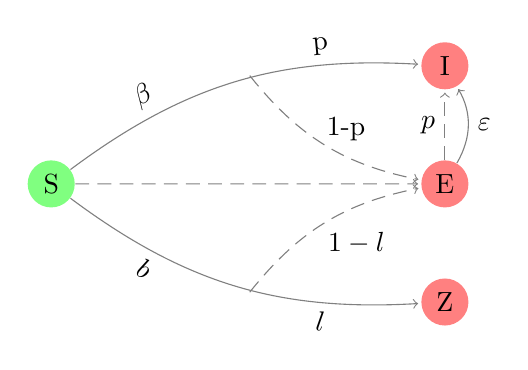
\begin{tikzpicture}[shorten >=1pt,->,draw=black!50, node distance=\layersep]
    \tikzstyle{every pin edge}=[<-,shorten <=1pt]
    \tikzstyle{neuron}=[circle,fill=black!25,minimum size=17pt,inner sep=0pt]
    \tikzstyle{input neuron}=[neuron, fill=green!50];
    \tikzstyle{output neuron}=[neuron, fill=red!50];
    \tikzstyle{miss node}=[inner sep=0,minimum size=1];
    % Draw the input layer nodes
     % This is the same as writing \foreach \name / \y in {1/1,2/2,3/3,4/4}
      \node[input neuron] (S) at (0,-2.5) {S};
      \node[ output neuron,  xshift=5cm,yshift=-1cm] (I) {I};
      \node[ output neuron,  xshift=5cm,yshift=-2.5cm] (E) {E};
      \node[ output neuron,  xshift=5cm,yshift=-4cm] (Z) {Z};
       \node[ miss node,  xshift=2.5cm,yshift=-1.1cm] (X) {};
       \node[ miss node,  xshift=2.5cm,yshift=-3.9cm] (X2) {};

	\path  (X) edge [dash pattern=on5pt off3pt,below, bend right=20] node [midway,right,xshift=-0.1cm,yshift=0.2cm]{1-p}(E) ;
 
      \path  (S) edge [above, bend left=20]node [sloped,near start,above] {$\beta$} node [sloped,near end,above] {p}  (I) ;
      \path  (E) edge [right, bend right=30] node [midway,right]{$\varepsilon $}(I) ;
      \path  (E) edge [dash pattern=on5pt off3pt] node [midway,left]{$p$}(I) ;
      \path  (S) edge [dash pattern=on5pt off3pt]  (E) ;
      \path  (S) edge [above, bend right=20]node [sloped,near start,below] {$b$} node [sloped,near end,below] {$l$}  (Z) ;
	\path  (X2) edge [dash pattern=on5pt off3pt,below, bend left=20] node [xshift=0.4cm]{$1-l $}(E) ;
	\end{tikzpicture}
   \caption{SEIZ Model}
\label{fig:SEIZ}
\end{figure}


\subsubsection{SpikeM model Features}
Kwon is another approach \cite{kwon2013prominent} discussing differences between the rumors' propagation pattern and the news events' propagation pattern on twitter.

SpikeM first was introduced by Yasuko Matsubara \cite{conf/kdd/MatsubaraSPLF12} which are used to describe the information diffusion. We present it as follow:
\begin{equation}
\Delta B(n + 1) =p(n + 1)\cdot( U(n) \cdot  \sum ^n_{t=n_b}(\Delta B(t) + S(t))\cdot f(n+1-t) + \varepsilon )
\end{equation}
\begin{equation}
p(n) = 1-\frac{1}{2}P_a(\sin (\frac{2\pi}{P_p} (n+P_s)))+1)
\end{equation}

\begin{equation}
U(n + 1)=U(n)-\Delta {B(n + 1) }
\end{equation}
where
\begin{equation}
f(\tau)=\beta \cdot \tau ^{-1.5}
\end{equation}
and initial conditions:
\begin{equation}
 \Delta B(0)=0 ,U(0) = N
\end{equation}
In addition, adding an external shock $S(n)$, a spike generated
at beginning time $n_b$. Mathematically, it is defined as follows:
\begin{equation}
S(n) =\begin{cases}0 &(n \neq n_b)\\S_b  & (n =n_b)\end{cases} 
\end{equation}
As the definition: 
\begin{equation}
B(n) + U(n) = N
\end{equation}
The term of $\sum ^n_{t=n_b}(\Delta B(t) + S(t))$ is the total number of informed blogers at time n,


\begin{table*}[!h]
 \centering
\scalebox{1}{
\begin{tabular}{@{\textbf{ }}lllllll@{}}
\toprule
\textbf{Symbol} & \textbf{Definition} \\ \midrule
N & total population of available bloggers\\ \midrule
$n_d$	&	duration of sequence\\
n	&	time-tick (n=0, . . . , $n_d$)\\\midrule
U(n)   &	count of \textbf{\underline{u}}n-informed bloggers\\
B(n)   &	count of informed \textbf{\underline{b}}loggers\\
$\Delta B(n)$	&	count of informed \textbf{\underline{b}}loggers at time n\\\midrule
f(n)   &	in\textbf{\underline{f}}ectiveness of a blog-post, at age n\\
$\beta$ & strength of infection\\
$\beta \cdot N$	&	"first-burst" size of infection\\\midrule
S(n)   &	volume of external \textbf{\underline{s}}hock at time n\\
$n_b$ & starting time of \textbf{\underline{b}}reaking news\\
$S_b$	&	strength of external shock at birth (time $n_b$)\\
$\varepsilon$	&	background noise \\\midrule
$P_a$ & strength of periodicity\\
$P_p$			& period\\
$P_s$			& phase shift of periodicity\\ \bottomrule


\end{tabular}}
\caption{Parameters of SpikeM}
\label{tab:Features_Impsortance}
\end{table*}


\subsubsection{Crowd Wisdom Features}
\subsubsection{CreditScore Features}

\newpage
\begin{table*}[!h]
\small
\centering
\scalebox{0.8}{
 \begin{tabular}{@{}lllllll@{}}
 \toprule
 \textbf{Category} & \textbf{Feature} & \textbf{Description}\\ \midrule
 Twitter Features& Hashtag & \% of the tweets containing \#hashtag\\
 		& Mention &  \% of the tweets mentioning others @user\\
 		& NumUrls &  \# of url in the tweet \\
 		& Retweets & average times of tweets have been retweeted \\ 
 		& Isretweet & \% of tweets are retweeted from others\\
 		& ContainNEWSWeb & \% of tweets containing URL and its domain's catalogue is News \\
 		& WotScore & average WOT score of domain in URL \\
 		& Isretweet & \% of tweets being retweeted from others\\
\midrule
 Text Features & LengthofTweet & average length of tweets\\
    & NumofChar & average number of individual characters of tweets\\
   & Capital &  average fraction of characters in Uppercase of tweets \\
   & Smile & \% of tweets containing :->, :-), ;->, ;-)\\
   & Sad & \% of tweets containing :-<, :-(, ;->, ;-(\\
   & NumPositiveWords & average number of positive words\\
   & NumNegativeWords & average number of negative words\\
   & Polarityscores & average polarity scores of the Tweets\\
   & Via & \% of tweets containing via\\
   & Stock & \% of tweets containing \$ \\
   & Question & \% of tweets containing ? \\
   & Exclamation & \% of tweets containing ! \\
   & QuestionExclamation & \% of tweets containing multi Question or Exclamation mark \\ 
   & I & \% of tweets containing first pronoun like I, my, mine, we, our   \\
   & You & \% of tweets containing second pronoun like U, you, your, yours \\ 
   & HeShe & \% of tweets containing third pronoun like he, she, they, his, etc. \\ \midrule
   User Features & Followers  & average number of followers\\
 	& Friends  & average number of friends\\
 	& Tweets  & average number of tweets being posted\\
 	& Numphoto  & average number of photos being posted\\
 	& IsInLargeCity  & \% of user living in large city\\
 	& Join\_date & average days since user joining Twitter\\
 	& Description  & \% of user having description\\
 	& Verified  & \% of user being a verified user\\
 	& ReputationScore & average ratio of \#Friends over (\#Followers + \#Friends)\\   \midrule
 Epidemiological Features & $\beta_{SIS}$ & average $\beta$ of Model SIS\\
 							& $\alpha_{SIS} $ & average $\alpha$ of Model SIS\\
 							& $\beta_{SEIZ}$ & average $\beta$ of Model SEIZ\\
 							& $b_{SEIZ}$ & average b of Model SEIZ\\
 							& $l_{SEIZ}$ & average l of Model SEIZ\\
 							& $\varepsilon$ & average $\varepsilon$ of Model SEIZ\\
 							& $\rho$ & average $\rho$ of Model SEIZ\\
 							& SEIZIndex & average SEIZIndex of Model SEIZ\\
		\midrule	
 SpikeM Model Features & $P_s$ & average $P_s$ of Model Spike\\
 							& $P_a$ & average $P_a$ of Model SpikeM\\
 							& $P_p$ & average $P_p$ of Model SpikeM\\
 							& $Q_s$  & average $Q_s$ of Model SpikeM\\
 							& $Q_a$ & average $Q_a$ of Model SpikeM\\
 							& $Q_p$ & average $Q_p$ of Model SpikeM\\ \midrule	
 Crowd Wisdom Features & Crowdwisdom & \% of tweets containing "Debunking Words"\\ \midrule
	
 Credit Score Features & CreditScore & average CreditScore\\
 \bottomrule
 \end{tabular}}
 \caption{Features of Time Series Rumor Detection Model}
 \label{tab:full_features}
\end{table*}
